\chapter{Anhang}\label{chp:Anhang}


\section{Bedienung}
Im Folgenden wird die Bedienung des Commute beschrieben. Dabei wird erst die Inbetriebnahme beschrieben, anschliessend der alltägliche Gebrauch und zuletzt wird erklärt, wie der Akku geladen werden kann.
\subsection*{Erste Inbetriebnahme}
Bei der ersten Inbetriebnahme des Commute muss der Magic Glove kalibriert werden. Insbesondere wird dabei die Ruhestellung der Hand definiert. Der Nutzer drückt drei Sekunden auf den Taster, dann zeigen die LEDs die Ruhestellung an. Das heisst, alle LEDs leuchten, diejenigen in der Mitte am stärksten. Nun hält der Nutzer seine Hand in Ruhestellung und zwar so, wie er gerne auf dem Longboard steht. Dies wird als Nullposition definiert. Anschliessend beginnen die LEDs der Reihe nach zu blinken – in eine Richtung führt der Nutzer dazu eine Bremsbewegung aus, in die andere Richtung die Bewegung, um zu Beschleunigen. Danach ist die Kalibration abgeschlossen. Nun kann das Commute genutzt werden.
\subsection*{Alltägliche Handhabung}
Auf dem Longboard befindet sich ein On/Off-Schalter, ebenso auf dem Magic Glove. Werden diese angeschaltet, ist das Commute betriebsbereit und der Nutzer kann losfahren. 
Entfernt sich der Nutzer mehr als drei bis vier Meter vom Bord, ist die Kommunikationsverbindung zwischen der Steuerung und der Antriebstechnik unterbrochen, und das Commute schaltet sich automatisch aus. Während der Fahrt wird dem Nutzer mithilfe der LEDs der Batteriestand des LiPo-Akkus angezeigt. Zudem wird die Batterie des Magic Gloves überwacht und auch über die LEDs angezeigt. 
\todo{ev. Ü'sicht der LEDs}
\subsection*{Akku aufladen}
Der Akku kann praktisch über einen Stecker am Longboard aufgeladen werden. Wie gesagt muss er dafür nicht herausgelöst werden. Während des Ladevorgangs zeigen drei LEDs am Longboard den Ladestand an. Diese LEDs leuchten auch kurz auf, wenn das Longboard eingeschaltet wird und zeigen damit den Akkustand. 


\section{Quellcode}
Der Quellcode ist unter folgenden Links aufrufbar.
\begin{center}
	\begin{tabular}{l|c}
		\hline 
		Hardware & https://github.com/noah95/skatemate-hw \\ \hline
		Software & https://github.com/noah95/skatemate-sw \\ \hline
	\end{tabular} 
\end{center}

Zusätzlich liegt er auf dem USB-Stick dieser Dokumentation bei.

\section{Schemati}
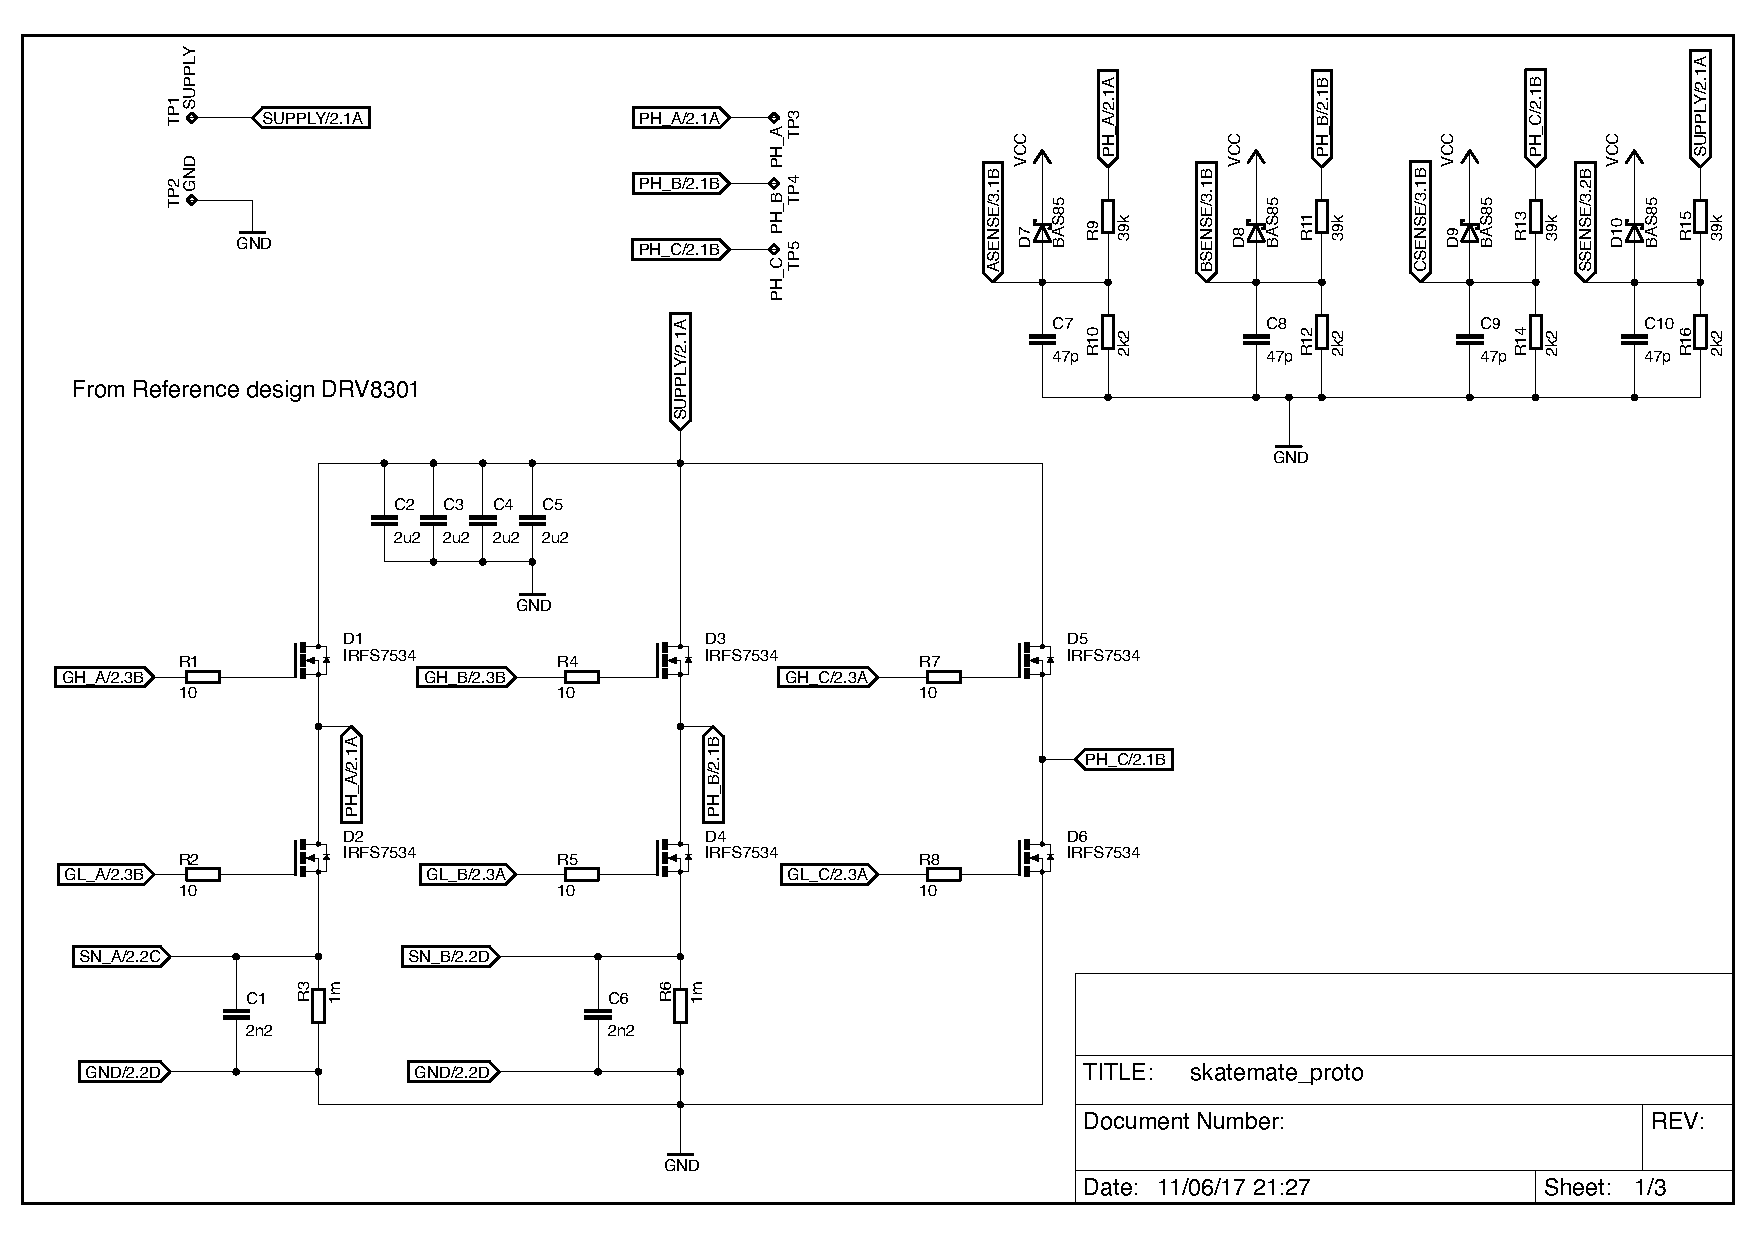
\includepdf[landscape, pages={1-3}]{1_Schema_Motorcontrol.pdf}
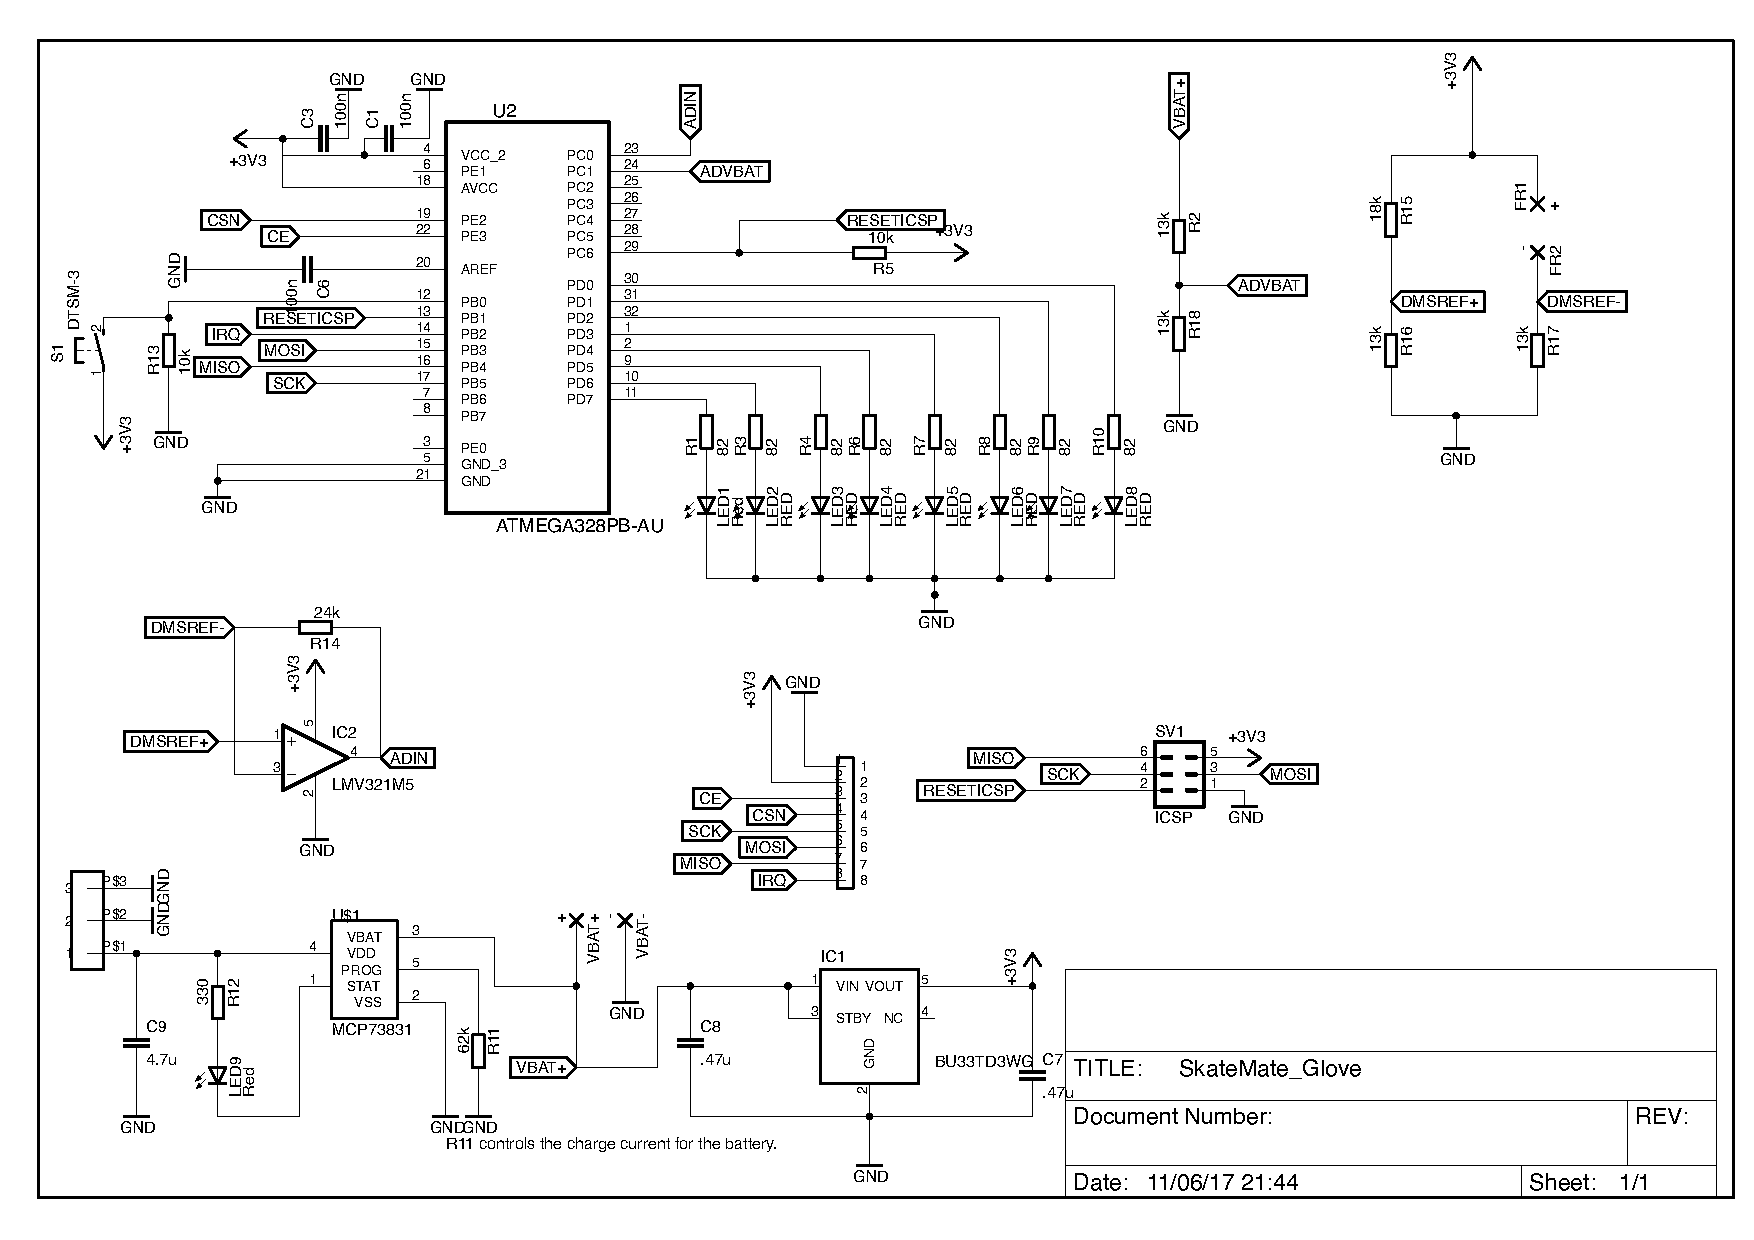
\includepdf[landscape, pages={1}]{2_Schema_Magic_Glove.pdf}
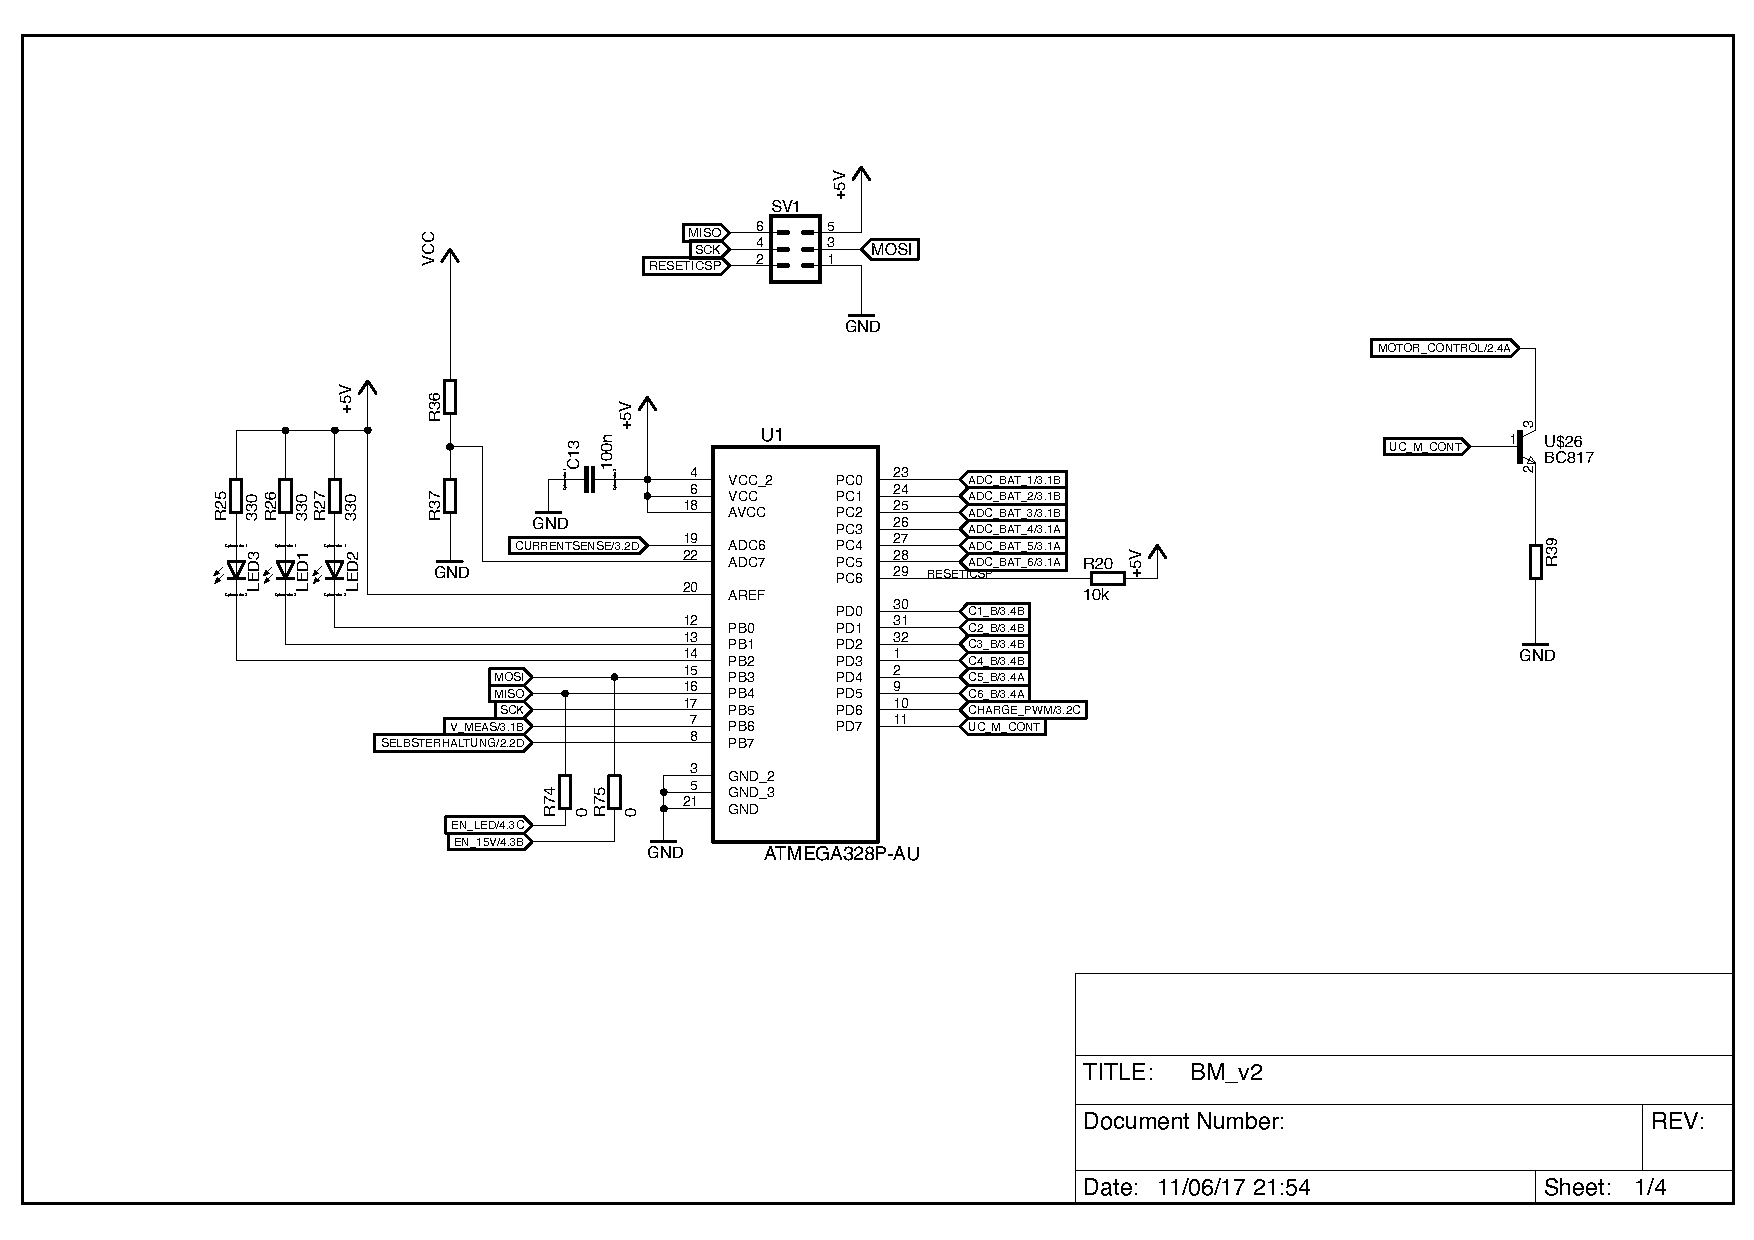
\includepdf[landscape, pages={1-4}]{3_Schema_Batter_Management.pdf}